\documentclass{article}

% ICLR 2026 submission template (single column, no strict page limit)
\usepackage{iclr2026_conference}

\usepackage[utf8]{inputenc} % allow utf-8 input
\usepackage[T1]{fontenc}    % use 8-bit T1 fonts
\usepackage{hyperref}       % hyperlinks
\usepackage{url}            % simple URL typesetting
\usepackage{booktabs}       % professional-quality tables
\usepackage{amsfonts}       % blackboard math symbols
\usepackage{amsmath}        % math
\usepackage{graphicx}       % figures
\usepackage{nicefrac}       % compact symbols for 1/2, etc.
\usepackage{xcolor}         % colors
\usepackage{times}          % restore Times font (matches NeurIPS look)

% Framework and module abbreviations
\newcommand{\dgtdm}{DG-TDM}
\newcommand{\modela}{MoDeA}
\newcommand{\tsa}{TSA}
\newcommand{\stg}{STG}

\title{DG-TDM: Dual-Granularity Temporal Dynamics Modeling with Spatial Prior Guidance for Fine-Grained Action Recognition}

\author{Anonymous Author(s) \\
  Paper under double-blind review}

\begin{document}

\maketitle

\begin{abstract}
Fine-grained action recognition requires distinguishing actions that look
nearly identical in single frames and differ mainly in how the body moves.
Two difficulties follow from this setting. Since all classes share a nearly
identical background, the action region must be located rather than inferred
from scene cues; and since the discriminating signal is motion, it must be
captured at two time scales, the short-term displacement of body parts over a
few frames and the long-term evolution of the whole sequence. We propose
\dgtdm, a three-branch framework that assigns these two requirements to
separate branches. A frozen CLIP encoder serves as a spatial expert, and a
spatio-temporal guidance (STG) branch injects its stable priors into a
lightweight 2D temporal encoder through bilateral window cross-attention and
adaptive gating, so that the encoder concentrates on the action region. The
core of the framework is a dual-granularity temporal dynamics module that
adds temporal modeling to the 2D backbone at the two time scales: the MoDeA
branch predicts dense cross-frame sampling offsets to follow short-term
body-part displacement, and the TSA branch maintains a long-term state
memory to model the sequence-level evolution. We evaluate the framework on
Diving48 and Something-Something V2 and use ablations to isolate the
contribution of each component.
\end{abstract}


\section{Introduction}
\label{sec:intro}

Fine-grained action recognition distinguishes actions that look nearly
identical in single frames and differ mainly in how the body moves. Recent
benchmarks drive the task toward this setting: Diving48 \cite{diving48}
separates dives by their rotation and timing, and Something-Something V2
\cite{goyal2017ssv2} separates everyday object manipulations by the direction
and manner of the motion, such as pushing something from left to right versus
from right to left. In both datasets, the classes are not separated by the
scene or by whole-body appearance but by how a small set of body parts moves
over time. On Diving48, for example, a $720^\circ$ rotation and a $900^\circ$
rotation of the same dive are two classes, yet every frame of the two videos
shows the same diver in the same poses against the same pool background; only
across frames does the rotation itself become visible.

This setting raises two problems. The first is spatial: since all classes
share the same background, the background carries no label-relevant
information and only distracts the model, so recognition must come from the
region where the body moves. The model thus has to know where to look before
it can read the motion. The second is temporal, and it spans two scales. On
the short scale, a class is often decided by a small local displacement over
a few frames, such as the path of a hand or the change in the angle of a limb.
The position that carries this detail moves from frame to frame, so a fixed
sampling grid loses it. On the long scale, the full meaning of an action is
determined by how the entire sequence evolves, so the model must maintain a
state over time rather than treat each frame in isolation. Both scales matter,
and dropping either one loses evidence that separates otherwise similar
classes.

Current video models only partially meet these needs. 3D CNNs
\cite{carreira2017slowfast,feichtenhofer2019slowfast} and video transformers
trained on large corpora
\cite{bertasius2021timesformer,liu2022videoswin,tong2022videomae,wang2024internvideo}
capture temporal structure, but they compute features at every position of
every frame, spending most of their capacity on background regions that carry
no signal; moreover, their sampling and attention are either too rigid to
follow a moving body part or too coarse to resolve a small displacement.
Deformable video transformers \cite{dvt2022} learn where to attend and perform
well on fine-grained benchmarks, but they select whole patches and therefore
miss the sub-window displacement that separates fine-grained classes. CLIP
\cite{radford2021clip} is strong precisely where the first problem lies:
pre-trained on massive image--text data, it judges reliably where people and
action-relevant content appear in a frame. Yet when CLIP is adapted to video,
either through frozen adapters \cite{lin2022evl} or end-to-end fine-tuning
\cite{rasheed2023vificlip}, the prior is absorbed into the encoder itself and
is not used to tell a separate recognition branch where the action is.
State-space models \cite{dao2023mamba,videomamba2024} aggregate long sequences
efficiently, but the spatial side remains open.

These observations suggest a division of labor. A frozen spatial expert
answers where the action is, and a trainable temporal encoder learns how it
moves. Because the expert is frozen, its positional judgment stays constant
throughout training and cannot overfit the background statistics of a small
fine-grained dataset; because the encoder is trained end-to-end, it can shape
its features around the motion. The two sides are complementary rather than
redundant.

Following this idea, we propose \dgtdm, a three-branch framework. A frozen
CLIP encoder serves as the spatial expert, and a spatio-temporal guidance
(STG) branch transfers its priors to the temporal encoder through bilateral
window cross-attention and adaptive gating, so that the encoder focuses on
the action region. The temporal encoder is built on a 2D ResNet backbone,
which has no temporal modeling of its own. We therefore insert, at every
stage, a dual-granularity temporal dynamics module (DG-TDM) that adds temporal
modeling on the 2D feature stream without inflating the backbone into a 3D
network. This module gives the overall framework its name, so we use the same
acronym for both throughout the paper. DG-TDM works at the two time scales of the motion: its MoDeA branch
predicts dense cross-frame sampling offsets to follow short-term body-part
displacement, and its TSA branch carries a long-term state memory over the
sequence to model how the action develops.

In summary, our main contributions are:
\begin{itemize}
  \item We propose \dgtdm, a three-branch framework for fine-grained action
  recognition that assigns localization to a frozen CLIP spatial expert and
  motion modeling to a trainable temporal encoder.
  \item We design a spatio-temporal guidance branch that injects the frozen
  priors into the temporal encoder through bilateral window cross-attention
  and adaptive gating, so that the encoder focuses on the action region.
  \item We develop a dual-granularity temporal dynamics module for the 2D
  backbone, in which MoDeA tracks short-term body-part displacement through
  dense deformable sampling and TSA models long-term evolution through a
  bidirectional state memory.
\end{itemize}


\section{Related Work}
\label{sec:related}

\textbf{Video modeling.}
Early approaches adapt image architectures to video by fusing frames at the
input or inflating convolutions to 3D \cite{tsm2018,carreira2017slowfast}.
Video transformers later replaced fixed kernels with self-attention, spanning
divided space-time attention in TimeSformer \cite{bertasius2021timesformer},
pooled multiscale attention in MViTv2 \cite{li2022mvitv2}, unified
convolution--attention designs in UniFormer \cite{li2022uniformer},
spatio-temporal focal modulation in Video-FocalNets \cite{videofocalnets2023},
and hierarchical windowed attention in Video Swin \cite{liu2022videoswin}.
On the training side, masked reconstruction \cite{tong2022videomae},
BERT-style video pretraining \cite{wang2022bevt}, and object-centric
attention \cite{orvit2022} enrich the learned representations, and general
video foundation models \cite{wang2024internvideo} scale this further. These
models are powerful but compute
features at every position of every frame, which is wasteful when only a
small region moves, as in fine-grained action. Deformable approaches instead
learn where to sample: the Deformable Video Transformer \cite{dvt2022}
dynamically predicts a small subset of video patches to attend, achieving
efficient temporal aggregation. Our MoDeA branch follows this direction but
predicts a dense 3D offset field and performs continuous trilinear sampling,
capturing sub-window motion that patch-level selection cannot represent.

\textbf{Adapters and parameter-efficient video models.}
Video adapters insert lightweight modules into a frozen encoder to adapt it
to a downstream task. ST-Adapter \cite{pan2022stadapter} pioneered this
direction for video, inserting space--time adapters between the blocks of a
frozen image backbone and showing that a small trainable footprint suffices
for recognition. This idea underlies EVL \cite{lin2022evl}, which
attaches temporal adapters to a fully frozen CLIP encoder, and AIM
\cite{yang2023aim}, which adapts an image backbone to video with
spatial--temporal modules and reaches competitive accuracy at a small
training cost. These designs keep the pretrained weights frozen and add a
small trainable footprint, which is valuable when fine-grained training data
is limited. We follow the same adapter-style residual design and extend it in
two respects: a dual-granularity temporal module that pairs local deformable
motion tracking with a long-term memory of the temporal response, and a
guidance branch that composes the frozen prior with a separate trainable
video backbone.

\textbf{State-space models and long-term temporal memory.}
Mamba \cite{dao2023mamba} models long sequences with a learned recurrent
state at linear cost, and video variants extend it along the temporal axis:
VideoMamba \cite{li2024videomamba} scans spatio-temporal tokens for efficient
video understanding, and a concurrent VideoMamba \cite{videomamba2024}
introduces a
bidirectional spatio-temporal selective scan. Our TSA branch shares the same
long-term memory intuition, carrying a state across the sequence to model the
overall response of an action, but instantiates it in a lightweight,
channel-wise form: a bidirectional linear recurrence with a per-channel decay,
used to produce a temporal channel gate rather than to replace the whole
architecture. This gives the model a cheap way to remember how each channel
responds over the whole action, complementing the local motion tracking of
MoDeA.

\textbf{Frozen vision-language priors.}
Contrastive image--text models such as CLIP \cite{radford2021clip} acquire
strong knowledge of where humans and action-relevant content appear, learned
from massive pre-training data. ViFi-CLIP \cite{rasheed2023vificlip} shows
that fine-tuning CLIP on videos transfers this knowledge effectively when
downstream data is scarce, while EVL \cite{lin2022evl} demonstrates the
frozen-encoder route. We follow the frozen route, since a frozen expert
guarantees positional judgments that never drift with the downstream task,
and we differ in how the prior is used: rather than absorbing the prior into
the encoder, we route it through a guidance branch that learns where and how
much to inject. The bilateral cross-attention lets the prior and the lower
branch refine each other, and the adaptive gate controls the amount of
injection per position, which is better suited to fine-grained tasks where
indiscriminate fusion can dilute the discriminative signal.

\textbf{Fine-grained action recognition.}
Fine-grained action recognition targets classes that differ in subtle body
movement rather than in scene \cite{diving48}. The difficulty
lies both in localizing the small moving region and in representing the fine
movement itself. Recent methods learn specialized spatio-temporal experts for
this task: DSTS \cite{li2022dsts} lets each stage specialize in the
discriminative spatio-temporal scales of a class, and TDN \cite{wang2021tdn}
models temporal difference at multiple scales. These methods focus on
temporal modeling but treat localization as an implicit side effect. Our
framework separates the two concerns explicitly: the frozen prior handles
localization through the guidance branch, while the dual-granularity module
handles representation through deformable motion and state aggregation.


\section{Method}
\label{sec:method}

We build the framework around two observations. Because the background is
shared across classes and carries no label-relevant information, the model
needs a reliable way to locate the action; because the classes differ in how
the body moves, the model must also capture the motion at both short and long
time scales. The framework, shown in Figure~\ref{fig:arch}, assigns these
needs to three cooperating branches: a frozen CLIP encoder that locates the
action, a spatio-temporal guidance (STG) block that transfers this knowledge
to the recognition branch, and a temporal action encoder, built on a 2D
ResNet backbone, that models the motion through its dual-granularity temporal
dynamics (DG-TDM) module. Figure~\ref{fig:stg} zooms in on the two core
blocks, STG and DG-TDM.

The data flow is as follows. Given $T$ sampled frames, the frozen CLIP
encoder extracts a patch map from each frame, and a lightweight alignment
module adapts it to the resolution of every backbone stage. The lower branch
is the recognition path: the 2D backbone extracts features stage by stage,
and after each of the four stages the STG block injects the aligned prior
into the features through bilateral window cross-attention, while the DG-TDM
module, inserted after the last bottleneck of the stage, adds temporal
modeling on the 2D feature stream. The final
stage feature is pooled and classified. The three branches divide the work
clearly: the frozen expert answers where the action is, the guidance decides
how much of this knowledge each position receives, and the temporal encoder
models how the action moves. The rest of this section details each part.

\begin{figure}[t]
  \centering
  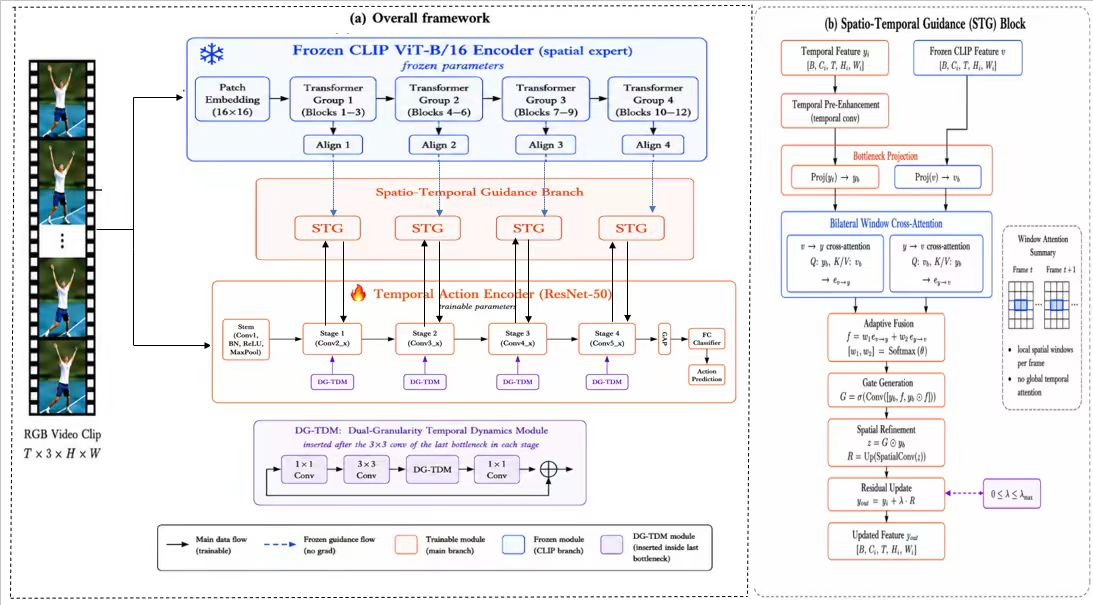
\includegraphics[width=\linewidth]{figures/dgtdm_stg_detail.jpg}
  \caption{Left: the dual-granularity temporal dynamics module (DG-TDM),
  composed of the MoDeA branch (motion deformation attention) and the TSA
  branch (temporal state aggregation). Right: the STG block with bilateral
  window cross-attention, adaptive fusion, and gated refinement.}
  \label{fig:stg}
\end{figure}

\noindent\textbf{Notation.}
Let a video be sampled into $T$ frames and processed by a 2D backbone with
$L$ stages. At stage $\ell$, the lower branch produces a feature map
$Y_\ell \in \mathbb{R}^{B \times C_\ell \times T \times H_\ell \times W_\ell}$,
where $B$ is the batch size and $(H_\ell, W_\ell)$ is the spatial resolution.
The frozen CLIP encoder produces a patch map
$V \in \mathbb{R}^{B \times 768 \times T \times 14 \times 14}$ that is aligned
to each stage resolution by a lightweight projection
$\mathrm{AuxAlign}_\ell(\cdot)$, yielding
$V_\ell \in \mathbb{R}^{B \times C_\ell \times T \times H_\ell \times W_\ell}$.
We use $\odot$ for element-wise multiplication and $\oplus$ for residual
addition, $\mathrm{DWConv}_T$ for a depth-wise convolution along time, and
$\mathrm{GAP}_{hw}$ for global average pooling over the spatial dimensions.

\subsection{Spatial prior and spatio-temporal guidance}
\label{sec:stg}

\textbf{Spatial prior.}
The upper branch is a frozen CLIP ViT-B/16 encoder \cite{radford2021clip}.
What we use is not object semantics but the spatial-position discriminability
acquired during pre-training: the encoder learns where humans, body parts,
and action-relevant objects tend to appear, and can judge, at each location,
whether the content belongs to the action or the background. The encoder
operates frame-wise: each frame passes through the ViT independently, the
class token is discarded, and the patch tokens form a 768-dimensional patch
map $V$ of resolution $14\times 14$. Since the encoder is frozen, this
positional knowledge enters as a stable prior that cannot be distorted by the
limited fine-grained training set. To make the prior available at every
stage, a lightweight alignment module $\mathrm{AuxAlign}_\ell$ interpolates
$V$ to
$(T, H_\ell, W_\ell)$ and applies a $1\times1\times1$ convolution, batch
normalization, and ReLU; the aligned prior $V_\ell$ feeds the guidance branch
below, and these alignment modules are the only trainable parameters attached
to the frozen encoder.

\textbf{Spatio-temporal guidance.}
The STG block is inserted after each temporal stage. Its purpose is to make
the lower branch attend to the action regions that the frozen encoder
identifies, so that the lower branch is not distracted by the background. We
use bilateral window cross-attention: information flows both from the prior
into the lower branch and from the lower branch into the prior, so that the
fusion is a mutual refinement rather than a one-way injection
(Figure~\ref{fig:stg}, right).

Given the lower-branch feature $Y_\ell$ and the aligned prior $V_\ell$, the STG
block first applies a light temporal convolution to $Y_\ell$ to pre-enhance
temporal cues, then projects both inputs into a shared bottleneck dimension
$C_\ell / r$ through separate $1\times1\times1$ convolutions:
\begin{equation}
  Y_b = \mathrm{Conv}^{1}_\mathrm{down}(Y_\ell), \qquad
  V_b = \mathrm{Conv}^{1}_\mathrm{down}(V_\ell).
\end{equation}
The projection to a lower dimension reduces the cost of the subsequent
attention and forces the two inputs to share a compact representation before
interaction.

We then compute bilateral window cross-attention within each local spatial
window. The window operation is confined to $w\times w$ neighborhoods in every
frame and never mixes across time, which keeps the cost linear in the spatial
resolution and preserves per-frame spatial structure: the feature is reshaped
into non-overlapping windows, the attention is applied inside each window, and
the result is restored to the original layout.

The first direction, $V \to Y$, treats $Y_b$ as queries and $V_b$ as keys and
values, letting the lower branch query the frozen prior:
\begin{equation}
  e_{V\to Y} = \mathrm{Softmax}\Big(\frac{Q_{Y} K_{V}^\top}{\sqrt{d}}\Big) V_{V},
  \qquad
  Q_{Y} = Y_b W_Q,\; K_{V} = V_b W_K,\; V_{V} = V_b W_V,
\end{equation}
where $W_Q, W_K, W_V$ are the query, key, and value projections and $d$ is the
head dimension. The second direction, $Y \to V$, reverses the roles and lets
the prior query the lower branch, so that the guidance reflects what the lower
branch has already learned:
\begin{equation}
  e_{Y\to V} = \mathrm{Softmax}\Big(\frac{Q_{V} K_{Y}^\top}{\sqrt{d}}\Big) V_{Y},
  \qquad
  Q_{V} = V_b W_Q,\; K_{Y} = Y_b W_K,\; V_{Y} = Y_b W_V.
\end{equation}
Multi-head attention is applied in both directions, with the query, key, and
value split across heads so that each head can attend to a different aspect of
the interaction.

The two directional outputs are combined by a learned softmax-weighted fusion
to adaptively balance the contribution of each direction. Rather than a fixed
average, we let the network learn the relative weight of the two directions,
which allows the guidance to be dominated by the prior when the lower branch
is uncertain and by the lower branch when it has learned reliable features:
\begin{equation}
  [w_1, w_2] = \mathrm{Softmax}(\beta), \qquad
  f = w_1 \, e_{V\to Y} + w_2 \, e_{Y\to V},
\end{equation}
where $\beta \in \mathbb{R}^2$ is initialized so that $w_1 = w_2 = 0.5$. A
gating network then decides, per spatial position, how much of the fused prior
should be applied to the lower branch. The gate takes the concatenation of
$Y_b$, the fused feature $f$, and their element-wise product, and outputs a
value in $(0,1)$:
\begin{equation}
  G = \sigma\big(\mathrm{Conv}\big([\,Y_b,\; f,\; Y_b \odot f\,]\big)\big).
\end{equation}
Including the product term $Y_b \odot f$ gives the gate access to the
interaction between the two inputs, enabling it to suppress positions where
they disagree. The gate is initialized with a negative bias, so that the
guidance is weak early in training and the lower branch can stabilize first.
The gated feature is refined by a spatial convolution and up-projected back to
the stage channel count, then added to the lower-branch feature with a bounded
residual scale $\lambda \in [0, \lambda_{\max}]$:
\begin{equation}
  \tilde{Y}_\ell = Y_\ell + \lambda \cdot \mathrm{Up}\big(G \odot Y_b\big).
\end{equation}
The scale $\lambda$ is a learnable scalar parameterized through a logit so
that it stays within $[0, \lambda_{\max}]$; it is initialized small to preserve
the identity at the start of training.

\subsection{Dual-granularity temporal dynamics module}
\label{sec:dgtdm}

\begin{figure}[t]
  \centering
  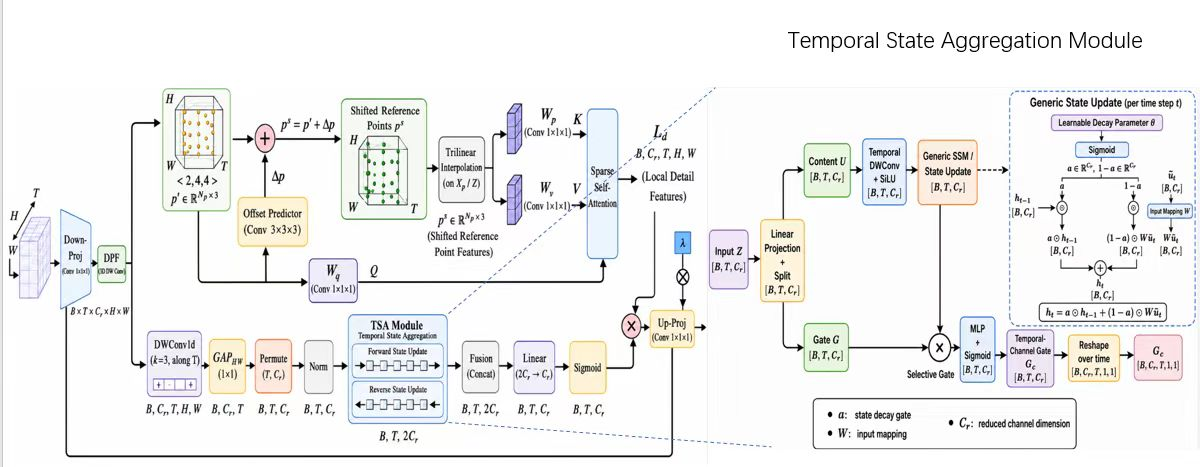
\includegraphics[width=\linewidth]{figures/arch_overview.jpg}
  \caption{Overall framework of \dgtdm. A frozen CLIP encoder extracts spatial
  priors from each frame; the spatial-temporal guidance (STG) branch injects
  these priors into a temporal action encoder through bilateral window
  cross-attention and adaptive gating. Inside each temporal stage, the
  dual-granularity temporal dynamics module (DG-TDM) refines the feature with a
  motion deformation attention (MoDeA) branch and a temporal state aggregation
  (TSA) branch.}
  \label{fig:arch}
\end{figure}

The lower branch is a temporal action encoder built on a 2D ResNet backbone.
A 2D backbone computes the feature of each frame independently and has no
temporal modeling of its own; rather than inflating it into a 3D network, we
insert the dual-granularity temporal dynamics module (DG-TDM)
(Figure~\ref{fig:stg}, left) after the $3\times3$ convolution of the last
bottleneck in each of the four stages. DG-TDM is a pseudo-temporal module: it
does not process frames jointly like a 3D convolution, but injects temporal
dynamics into the 2D features through deformable cross-frame sampling and a
temporal state scan, leaving the backbone structure and its pretrained weights
intact. The module models the motion at the two time scales identified in the
introduction. MoDeA handles the short-term part: it predicts where to sample
across frames to follow the displacement of a body part over successive
frames. TSA handles the long-term part: it carries a state over the whole
sequence and models how the overall temporal response of the action develops.
Together they let the lower branch represent the fine movements that
distinguish fine-grained actions.

\subsubsection{Adapter-style formulation}
\label{sec:adapter}

Following an adapter-style residual design, the DG-TDM block first projects the
stage feature into a compact bottleneck dimension $C_\ell / r$, then applies
the two motion branches, and finally projects back and adds a residual. To
preserve the identity at initialization, the output projection is zero-initialized
and a learnable scalar scale is applied. The structure is
\begin{align}
  X_d &= \mathrm{Down}(X), \label{eq:down}\\
  X_p &= X_d + \mathrm{DPE}(X_d), \label{eq:dpe}\\
  L_d &= X_p + \mathrm{MoDeA}\big(\mathrm{LN}(X_p)\big), \label{eq:modelocal}\\
  \tilde{G}_c &= \mathrm{TSA}\big(\mathrm{GAP}_{hw}\circ \mathrm{DWConv}_T(X_p)\big),
       \label{eq:tsagate}\\
  \tilde{X} &= X + s \cdot \mathrm{Up}\big(\tilde{G}_c \odot L_d\big),
       \label{eq:adapterout}
\end{align}
where $\mathrm{Down}$ and $\mathrm{Up}$ are $1\times1\times1$ convolutions,
$\mathrm{DPE}$ is a depth-wise $3\times3\times3$ convolution that injects
dynamic position information, $\mathrm{LN}$ is layer normalization applied per
spatial--temporal position, $\mathrm{DWConv}_T$ is a depth-wise convolution
along time, $\mathrm{GAP}_{hw}$ is global average pooling over the spatial
dimensions, and $s$ is the learnable scale. We describe $\mathrm{MoDeA}$ and
$\mathrm{TSA}$ next.

The bottleneck design keeps the DG-TDM cheap: the two motion branches operate
in $C_\ell / r$ channels rather than $C_\ell$, and the output projection is
zero-initialized so that the block behaves as an identity at the start of
training. This is important for fine-grained tasks because it lets the
pretrained backbone be reused directly and adds only a small trainable
footprint; it also stabilizes early optimization, since the block initially
passes the stage feature through unchanged and only gradually learns to add
motion-aware refinements. The two branches read the same projected input
$X_p$ but in different ways: MoDeA operates on the full spatio-temporal
tensor and refines it locally, while TSA pools the spatial dimensions first
and returns a compact per-channel gate. The gate is applied to the MoDeA
output $L_d$ before the up-projection, so the two branches interact as a
product: the local motion details are kept only where the temporal memory
indicates that the channel matters for the action.

\subsubsection{Motion deformation attention (MoDeA)}
\label{sec:modela}

Actions are, by definition, movements of body parts relative to one another:
a hand travels from the upper-left corner of the frame to somewhere else, and
the trajectory of that movement is what distinguishes one action from another.
A key consequence is that the position of the action content is \emph{not}
fixed across frames: the location that carries the discriminative detail at
time $t$ holds different, irrelevant content by time $t+1$. A feature sampled
on a fixed grid therefore loses the motion, because it keeps sampling the same
coordinates while the content has moved away. MoDeA addresses this by
predicting, at each spatio-temporal position, a deformation offset that tracks
where the relevant content has moved, and then attending over the displaced
sampling positions. This follows the line of deformable video transformers
\cite{dvt2022}, which select the patches to attend based on motion, but differs
in that MoDeA predicts a dense 3D offset field and performs continuous
trilinear sampling, giving a finer representation of local motion than
patch-level selection.

Formally, let $Z = \mathrm{LN}(X_p)$ denote the layer-normalized input of
shape $[B, C_r, T, H, W]$, where $C_r = C_\ell / r$. The branch first projects
the query from $Z$:
\begin{equation}
  Q = Z W_Q,
\end{equation}
with $W_Q$ a $1\times1\times1$ convolution. The query is then split into
$G$ channel groups, and each group produces a deformation field through a
depth-wise 3D convolution followed by layer normalization, GELU, and a
point-wise convolution that outputs three channels:
\begin{equation}
  \widehat{\Delta p} = \mathrm{Conv}_{1\times1}\Big(\mathrm{GELU}\big(
      \mathrm{LN}\big(\mathrm{DWConv}_{3d}(Q)\big)\big)\Big),
\end{equation}
where $\widehat{\Delta p} \in \mathbb{R}^{B\cdot G \times 3 \times T_p \times H_p \times W_p}$
encodes offsets $(\Delta z, \Delta y, \Delta x)$ at the down-sampled lattice
$(T_p, H_p, W_p)$. The raw offsets are passed through tanh and scaled so that
the sampling stays stable:
\begin{equation}
  \Delta p = \mathrm{tanh}\big(\widehat{\Delta p}\big) \odot \rho,
  \qquad
  \rho_d = \min\Big(1,\ \frac{f}{S_d}\Big),
\end{equation}
where $S_d$ is the lattice size along dimension $d$ and $f$ is a scaling factor.
This bounds the displacement to a fraction of the lattice, preventing the
sampling from drifting too far from the reference.

A reference grid $p$ is defined on the down-sampled spatio-temporal lattice,
normalized to $[-1, 1]$, and expanded over the batch and groups:
\begin{equation}
  p_{ijk} = \Big(\frac{2 i}{T_p}-1,\; \frac{2 j}{H_p}-1,\; \frac{2 k}{W_p}-1\Big).
\end{equation}
The actual sampling positions are $p' = p + \Delta p$. The input feature is
sampled at $p'$ with trilinear interpolation:
\begin{equation}
  X_s = \mathrm{GridSample}\big(Z,\; p'\big),
\end{equation}
which yields the sampled feature $X_s$ at the deformed positions. Because
sampling is continuous, $X_s$ captures motion that falls between grid cells.

The sampled features are projected into keys and values, and a multi-head
attention is computed between the full query positions and the sampled
positions:
\begin{equation}
  \mathrm{MoDeA}(Z) = \mathrm{Softmax}\Big(\frac{Q K^\top}{\sqrt{d}}\Big) V_a,
\end{equation}
with $Q$ from $Z$, and $K$ and $V_a$ from $X_s$. The attention aggregates the
sampled positions for every query, letting each query collect motion-deformed
context.

Because each group has its own displacement field, different groups can
specialize to different motion directions or magnitudes. One group may track a
fast-moving hand while another tracks a slowly translating torso, and the
attention over the group-specific sampled positions integrates the context
that each group needs. Because
the offsets are predicted from the data itself, no supervision or optical flow
is required; the deformation emerges purely from the recognition objective.
This branch is what gives the lower branch the ability to represent motion
change: it turns the fixed-grid feature into one that actively follows where
the informative content has moved between frames.

\subsubsection{Temporal state aggregation (TSA)}
\label{sec:tsa}

The long scale calls for a different mechanism. Two classes may share the
same short-term displacement pattern and differ only in how their responses
accumulate over the entire sequence, and this difference is exactly what a
local sample cannot reveal. TSA therefore maintains a state over time and
aggregates evidence across all frames rather than within a local
neighborhood. It is built as a lightweight selective state-space module
(Figure~\ref{fig:stg}, left, bottom-right). In brief, it
splits the channel-wise temporal signal into a content stream $U$, which the
state update accumulates into memory, and a selection gate $G$, which decides
what is kept; the content stream passes through a bidirectional state update
whose learnable decay controls the memory horizon, the state output is
multiplied by the gate, and the result becomes a temporal channel gate that
reweights the lower-branch feature.

\noindent\textbf{Linear projection and split.}
Given the input $Z \in \mathbb{R}^{B \times T \times C_r}$ (after spatial
pooling and a normalization), TSA first applies a linear projection and splits
the output along the channel dimension into two equal streams:
\begin{equation}
  [\,U,\; G\,] = \mathrm{Split}\big(\mathrm{Linear}(Z)\big),
  \qquad U, G \in \mathbb{R}^{B \times T \times C_r}.
\end{equation}
The two streams play complementary roles. The content stream $U$ is the
signal to be memorized: it is what the state update accumulates over time, so
after the recurrence, $U$ determines what the long-term memory contains. The
gate stream $G$ is the selector: it decides, at each time step and for each
channel, how much of the memorized content is kept. Splitting one projection
into both lets them specialize: $U$ learns an input that aggregates well over
time, while $G$ learns an input that marks the time steps worth keeping.

\noindent\textbf{Context enhancement.}
The content stream $U$ is first passed through a depth-wise temporal
convolution and a SiLU activation to produce the context $\tilde{U}$:
\begin{equation}
  \tilde{U} = \mathrm{SiLU}\big(\mathrm{DWConv}_T(U)\big),
  \qquad \tilde{U} \in \mathbb{R}^{B \times T \times C_r}.
\end{equation}
The depth-wise temporal convolution mixes nearby time steps so that each input
to the state update sees a small neighborhood, while the SiLU activation
keeps the magnitude under control for the recurrent scan.

\noindent\textbf{Bidirectional state update with learnable decay.}
The context is scanned forward and backward over time by a state-space
recurrence. At each time step $t$, a learnable decay $a \in (0,1)^{C_r}$
controls how much of the previous state is retained. The decay is produced
from a learnable parameter $\theta$ and a non-negative scalar $\xi$,
\begin{equation}
  a = \sigma(\theta \cdot \xi), \qquad 1 - a = e^{-\xi},
\end{equation}
so that $a$ and $1-a$ are coupled and both lie in $(0,1)$. The forward and
backward states are updated by
\begin{align}
  h_t^f &= a \odot h_{t-1}^f + (1 - a) \odot W \tilde{u}_t,
          & h_0^f &= 0, \label{eq:tsa_fwd}\\
  h_t^b &= a \odot h_{t+1}^b + (1 - a) \odot W \tilde{u}_t,
          & h_{T+1}^b &= 0, \label{eq:tsa_bwd}
\end{align}
where $W$ is a learnable input mapping and $\tilde{u}_t$ is the context at
time $t$. The forward state accumulates information causally from the past,
and the backward state accumulates from the future; together they cover the
entire temporal context. The learnable decay $a$ gives the state a
controllable memory horizon: when $a$ is close to $1$ the state retains most
of its history (long memory), and when $a$ is close to $0$ the state is
dominated by the current input (short memory).

\noindent\textbf{Selective gate.}
The two states are concatenated along the channel dimension,
\begin{equation}
  h_t = \big[\, h_t^f;\; h_t^b \,\big] \in \mathbb{R}^{B \times T \times 2 C_r},
\end{equation}
and then element-wise multiplied by the gate stream $G$, giving a selectively
gated content
\begin{equation}
  h_t^{\mathrm{sel}} = h_t \odot G.
\end{equation}
The multiplication by $G$ is what makes the module selective rather than a
plain linear recurrence: at each time step, the gate stream decides which
channels of the processed state should contribute, so the model can emphasize
time steps that look relevant and suppress ones that look noisy.

\noindent\textbf{Temporal channel gate and reshape.}
The selectively gated content is passed through an MLP and a sigmoid to
produce the temporal channel gate,
\begin{equation}
  G_c = \sigma\big(\mathrm{MLP}(h_t^{\mathrm{sel}})\big)
  \in \mathbb{R}^{B \times T \times C_r}.
\end{equation}
Finally, $G_c$ is reshaped to the spatial layout of the lower-branch feature,
\begin{equation}
  \tilde{G}_c = \mathrm{Reshape}(G_c) \in \mathbb{R}^{B \times C_r \times T \times 1 \times 1},
\end{equation}
so that it can be broadcast-multiplied with the spatial feature $L_d$ in
Equation~\eqref{eq:modelocal}. The gate $G_c$ reweights the locally refined
motion feature: it amplifies channels whose long-term temporal response
indicates the action and suppresses channels that respond only to static
appearance, letting the aggregated state memory influence which motion
features the final representation keeps.

\noindent\textbf{Discussion.}
TSA combines three ingredients that are usually studied separately: a content
stream, an input-dependent selection gate, and a long-term state memory with a
learnable decay. The selective multiplication by $G$ implements the
input-dependent selection that distinguishes Mamba-style selective state-space
models from plain linear recurrences, while the learnable decay $a$ gives the
state a controllable memory horizon. The whole module operates in the
reduced bottleneck dimension $C_r$, so its cost is linear in the sequence
length and its parameter footprint is small. The mechanism is related to
recent state-space video models \cite{videomamba2024} in spirit, but here it
produces only a temporal channel gate rather than a full feature, so it does
not need the heavy selective scan machinery used in those models.

The two branches complement each other. MoDeA operates at the short time scale
and on spatial positions: it returns a refined local feature that carries the
fine motion of individual body parts. TSA operates at the long time scale and
on channels: it returns a per-channel gate that carries how the action's
overall response develops. Each branch is incomplete on its own. Short-term
deformation without long-term context cannot tell whether a movement is a
transient jitter or a sustained part of the action, and long-term memory
without short-term refinement cannot distinguish actions whose overall response
is similar but whose local motion differs. Their product combines both views:
the gate $G_c$ selects, channel by channel, which parts of the locally refined
motion feature contribute to the final representation, which is then
up-projected and added to the stage feature.

\subsection{Complexity and training}
\label{sec:complexity}

The framework keeps the additional cost over a plain 2D backbone modest. The
frozen CLIP encoder runs without gradients and is shared across all stages,
so it contributes only forward-pass cost. The STG block operates in a reduced
bottleneck dimension
and confines attention to local windows, so its cost per stage is
$O\big(B \cdot C_r \cdot T \cdot H \cdot W \cdot w^2\big)$, linear in the
spatial resolution. The MoDeA branch samples a down-sampled lattice, so its
attention cost is proportional to the number of sampled positions rather than
the full resolution, and the TSA branch is linear in $T$. Because the two
motion branches operate in the bottleneck and never materialize a
full-resolution intermediate tensor, both parameters and memory stay low; we
report concrete counts in the appendix.

The final stage feature is pooled spatially and temporally and passed to a
linear classifier. We train end-to-end with a label-smoothed cross-entropy
loss. Smoothing softens the target distribution and prevents over-confidence on
classes that are visually close, a common failure mode in fine-grained
recognition where two classes may share nearly identical poses. Formally, the
target $\tilde{y}$ mixes the one-hot label $y$ with a uniform distribution,
\begin{equation}
  \tilde{y}_c = (1 - \varepsilon)\, y_c + \frac{\varepsilon}{K},
\end{equation}
where $K$ is the number of classes and $\varepsilon$ the smoothing factor. The
frozen encoder, the alignment modules, the STG blocks, and the DG-TDM blocks
are trained jointly, with the frozen branch kept at zero gradient.


\section{Experiments}
\label{sec:experiments}

We evaluate \dgtdm on two motion-centric action recognition benchmarks,
Diving48 and Something-Something V2 (SSv2). Below we first describe the
datasets, evaluation protocol, and implementation details, then compare
\dgtdm with existing methods on the two benchmarks, and finally present
ablation studies on Diving48 that isolate the contribution of each branch.

\subsection{Setup}
\label{sec:setup}

\textbf{Datasets.}
We evaluate on two benchmarks. Diving48 \cite{diving48} contains approximately
$18$k trimmed video clips of $48$ dive classes; its videos share similar pool
backgrounds and differ in subtle body movements such as rotation angle and
timing. We use the official V2 train/test split. Something-Something V2
\cite{goyal2017ssv2} is a large-scale motion-centric benchmark of around $220$k
videos in $174$ classes of everyday object manipulations, such as pushing,
pulling, and dropping; the classes are defined by the direction and manner of
the motion rather than by the objects or the scene, so success requires
temporal reasoning over the whole sequence. For both datasets we report top-1
and top-5 accuracy.

\textbf{Implementation details.}
We use a ResNet-50 backbone as the temporal action encoder. The frozen spatial
branch is a CLIP ViT-B/16 encoder whose parameters are kept frozen. The DG-TDM
module is inserted after the $3\times3$ convolution of the last bottleneck in
each of the four stages, with a reduction ratio of $4$; the STG block is
inserted after each of the four stages, with a window size of
$7$. We train with stochastic gradient descent, momentum $0.9$, weight decay
$5\times10^{-4}$, and a step schedule. The classifier uses label-smoothed
cross-entropy with smoothing $0.1$. Training is performed on two NVIDIA
V100-SXM2-32GB GPUs. Our main setting samples $T=8$ frames per video. Full
hyperparameters are listed in the appendix.

\textbf{Baselines.}
We compare against representative methods that report results on Diving48 and
SSv2. Reported numbers of the compared methods are taken from their original
papers (with the source cited in the table).

\subsection{Comparison with state of the art}
\label{sec:main}

Tables~\ref{tab:diving48} and \ref{tab:ssv2} compare \dgtdm with existing
methods on the two benchmarks. We report values exactly as published in the
original papers, together with the input configuration (frames $\times$
resolution) used by each method. The compared methods span specialized
fine-grained models (DSTS, CAN), lightweight 2D temporal models (TANet,
TEINet, GST, AdaFuse, TDN, and AK-Net), and recent adaptation baselines
(MANet, LoKi, and AIM). For Diving48, the numbers under the DSTS protocol
are as reported by DSTS
\cite{li2022dsts} and those under the DVT protocol by DVT \cite{dvt2022}; the
remaining rows come from the original publications. For SSv2, all baseline values are taken from the cited original papers and
are restricted to configurations with an explicitly reported $8$-frame input.
We evaluate \dgtdm on both benchmarks with $8$ frames.

\begin{table}[t]
  \centering
  \caption{Comparison on Diving48. Metrics are top-1 and top-5 accuracy (\%).
  The Input / views column preserves the notation used by each source: an
  explicit $frames\times clips\times crops$ value is shown when reported,
  while sources that report only the number of input frames retain a single
  frame-count value. Resolution-based configurations are also kept in their
  original form. Top-5 values are marked ``-'' where the source does not
  report them. ``$\dagger$'' marks the DSTS protocol
  \cite{li2022dsts} and ``$\ddagger$'' the DVT protocol \cite{dvt2022}; the
  two papers use different evaluation protocols, so values across the two
  groups are not directly comparable. The TDN row reports the corrected
  official result compiled in \cite{chen2022aknet}, using the updated
  Diving48 annotations. The CAN row takes the $8$-frame ablation
  configuration from \cite{li2025can}, whose main result uses $16$ frames;
  the AIM row reports the $8$-frame result reproduced by \cite{cai2025loki}.}
  \label{tab:diving48}
  \small
  \begin{tabular}{llccc}
    \toprule
    Method & Backbone & Input / views & Top-1 (\%) & Top-5 (\%) \\
    \midrule
    \multicolumn{5}{l}{\emph{Protocol of DSTS \cite{li2022dsts}}} \\
    Video Swin-B \cite{liu2022videoswin} & Swin-B & - & 80.5$\dagger$ & - \\
    Swin-B + DSTS \cite{li2022dsts} & Swin-B & - & 83.0$\dagger$ & - \\
    \midrule
    \multicolumn{5}{l}{\emph{Protocol of DVT \cite{dvt2022}}} \\
    DVT \cite{dvt2022} & ViT-B & 16$\times$224$^2$ & 83.5$\ddagger$ & - \\
    \midrule
    \multicolumn{5}{l}{\emph{Methods with lightweight backbones}} \\
    TDN \cite{wang2021tdn} (corrected) & ResNet-50 & 8 & 80.5 & - \\
    AK-Net (TSM) \cite{chen2022aknet} & ResNet-50 & 8 & 79.3 & - \\
    AK-Net (TDN) \cite{chen2022aknet} & ResNet-50 & 8 & 81.7 & - \\
    CAN \cite{li2025can} (8-frame config) & ResNet-50 & 8$\times1\times1$ & 82.7 & 98.3 \\
    MANet \cite{li2025manet} & ResNet-50 & 8$\times1\times1$ & 81.8 & 98.0 \\
    LoKi \cite{cai2025loki} & ViT-B/16 & 8$\times1\times1$ & 78.4 & 98.2 \\
    AIM \cite{yang2023aim} & ViT-B/16 & 8$\times1\times1$ & 77.4 & 97.8 \\
    \midrule
    \multicolumn{5}{l}{\emph{Ours}} \\
    \dgtdm & ResNet-50 + frozen CLIP & 8$\times1\times1$ & \textbf{83.55} & \textbf{97.82} \\
    \bottomrule
  \end{tabular}
\end{table}

\begin{table}[t]
  \centering
  \caption{Comparison on Something-Something V2 with $8$ input frames and
  lightweight ResNet-50 backbones. Metrics are top-1 and top-5 accuracy (\%).
  TANet follows its original $8\times1\times1$ protocol \cite{liu2021tam};
  TDN and AK-Net follow the unified $8$-frame comparison in AK-Net Table II
  \cite{chen2022aknet}; ILA, STAN-conv, and M2-CLIP follow their reported
  multi-view 8-frame settings \cite{tu2023ila,liu2023stan,wang2024m2clip}.
  FEASE-Net, CAN, and MANet use their reported $8\times1\times1$
  configurations \cite{zhou2024fease,li2025can,li2025manet}. A dash denotes
  a top-5 value not reported by the source.}
  \label{tab:ssv2}
  \small
  \begin{tabular}{llccc}
    \toprule
    Method & Backbone & Frames & Top-1 (\%) & Top-5 (\%) \\
    \midrule
    \multicolumn{5}{l}{\emph{ResNet-50 and lightweight baselines}} \\
    TANet \cite{liu2021tam} (IN) & ResNet-50 & 8$\times1\times1$ & 60.5 & 86.2 \\
    TEINet \cite{liu2020teinet} (IN) & ResNet-50 & 8$\times1$ & 61.3 & - \\
    GST \cite{luo2019gst} (IN) & ResNet-50 & 8$\times1$ & 61.6 & - \\
    AdaFuse \cite{meng2021adafuse} (IN) & ResNet-50 & 8$\times1$ & 59.8 & - \\
    TDN \cite{wang2021tdn} (IN, corrected) & ResNet-50 & 8$\times1$ & 64.0 & - \\
    AK-Net (TSM) \cite{chen2022aknet} (IN) & ResNet-50 & 8$\times1$ & 60.2 & - \\
    AK-Net (TDN) \cite{chen2022aknet} (IN) & ResNet-50 & 8$\times1$ & 64.3 & - \\
    \midrule
    \multicolumn{5}{l}{\emph{Recent 8-frame adaptation baselines}} \\
    ILA \cite{tu2023ila} (ViT-B/16) & ViT-B/16 & 8$\times4\times3$ & 65.0 & 89.2 \\
    STAN-conv \cite{liu2023stan} (CLIP) & ViT-B/16 & 8$\times1\times3$ & 65.2 & 90.5 \\
    M2-CLIP \cite{wang2024m2clip} (CLIP) & ViT-B/16 & 8$\times1\times3$ & 66.9 & 90.1 \\
    FEASE-Net \cite{zhou2024fease} & ResNet-50 & 8$\times1\times1$ & 64.2 & 88.8 \\
    CAN \cite{li2025can} & ResNet-50 & 8$\times1\times1$ & 63.9 & 89.1 \\
    MANet \cite{li2025manet} & ResNet-50 & 8$\times1\times1$ & 63.6 & 88.8 \\
    \midrule
    \dgtdm (ours) & ResNet-50 + frozen CLIP & 8$\times1\times1$ & \textbf{65.3} & \textbf{89.1} \\
    \bottomrule
  \end{tabular}
\end{table}

Under the $8\times1\times1$ single-clip protocol, \dgtdm reaches
$83.55\%$/$97.82\%$ top-1/top-5 on Diving48 and $65.3\%$/$89.1\%$ on SSv2.
Its top-1 accuracy is the highest among the compared methods with a ResNet-50
backbone on both benchmarks.

\subsection{Ablation studies}
\label{sec:ablation}

We ablate \dgtdm on Diving48, the benchmark whose classes share the most
similar backgrounds and therefore stresses localization the most. All
ablations use $8$ frames. We organize the analysis into three parts: the
progressive build-up of the framework (Table~\ref{tab:ablation}), the
internal design choices of each branch (Table~\ref{tab:design}), and the
sensitivity to the main hyperparameters (Table~\ref{tab:hyper}).

\textbf{Progressive build-up.}
Table~\ref{tab:ablation} adds the components of \dgtdm to a TSN-style
baseline (a plain ResNet-50 that samples frames, extracts 2D features, and
classifies their temporal average), one component at a time, using the
$8\times1\times1$ protocol of the main comparison. Each step isolates one
mechanism: MoDeA contributes short-term cross-frame alignment, TSA adds a
persistent long-term state and thereby completes DG-TDM, and the STG branch
finally brings in the frozen-CLIP prior as guidance.

\begin{table}[t]
  \centering
  \caption{Progressive ablation on Diving48 with $8\times1\times1$ views.
  Each row adds one component of \dgtdm to the previous configuration; the
  last column reports the top-1 gain over the preceding row. Metrics are
  top-1 and top-5 accuracy (\%).}
  \label{tab:ablation}
  \small
  \begin{tabular}{lccc}
    \toprule
    Configuration & Top-1 (\%) & Top-5 (\%) & $\Delta$Top-1 \\
    \midrule
    TSN-style baseline (ResNet-50) & 71.36 & 95.82 & --- \\
    + MoDeA (short-term motion alignment) & 79.09 & 96.74 & +7.73 \\
    + TSA (long-term state memory; DG-TDM complete) & 81.57 & 97.77 & +2.48 \\
    + STG guidance (full \dgtdm) & \textbf{83.55} & \textbf{97.82} & +1.98 \\
    \bottomrule
  \end{tabular}
\end{table}

MoDeA raises top-1 by $7.73$ points over appearance averaging alone,
confirming that following the moving body part across frames is essential
when the discriminative signal is a small local displacement. TSA adds a
further $2.48$ points, showing that a state that aggregates the whole
sequence captures information that local alignment leaves out. The STG
branch contributes the final $1.98$ points, which measures the value of
bilateral interaction and adaptive gating under the same temporal encoder.
Top-5 accuracy improves consistently along the sequence, with the full model
reaching $97.82\%$.

\textbf{Design choices.}
Table~\ref{tab:design} switches off one internal design choice at a time
from the full model, so that each row keeps the affected component present
and isolates a single factor. The overall contribution of the MoDeA branch
is already measured by Table~\ref{tab:ablation} (removing it recovers the
$+7.73$ points of the baseline row), so the rows below address the choices
inside the remaining machinery. One factor is the fusion of the two DG-TDM
branches, which are combined multiplicatively so that TSA selects the
MoDeA-refined local features with a per-channel gate; we compare this with
adding the two branch outputs in parallel. A second factor is the direction
of the TSA scan, and we remove its backward pass. The bilateral nature of
the STG guidance is a third factor, and we keep only the prior-to-feature
direction. The last factor is where the frozen CLIP prior is applied: we
test injecting it at the last stage only, asking whether the position
knowledge must be used progressively at several spatial scales or once at
the top. The full model serves as the reference row.

\begin{table}[t]
  \centering
  \caption{Design-choice ablation on Diving48 with $8\times1\times1$ views.
  Each row switches off one internal design choice of the full \dgtdm while
  keeping the affected component and the remaining configuration fixed.
  Metrics are top-1 and top-5 accuracy (\%).}
  \label{tab:design}
  \small
  \begin{tabular}{lcc}
    \toprule
    Configuration & Top-1 (\%) & Top-5 (\%) \\
    \midrule
    Full \dgtdm (reference) & \textbf{83.55} & \textbf{97.82} \\
    DG-TDM: additive branch outputs (w/o TSA gate selection) & 83.41 & 98.02 \\
    TSA: forward-only scan (w/o backward context) & 82.58 & 97.76 \\
    STG: one-directional guidance (w/o $Y\!\to\!V$) & 82.70 & 97.88 \\
    CLIP prior: last-stage-only guidance (w/o per-stage) & 81.83 & 97.65 \\
    \bottomrule
  \end{tabular}
\end{table}

\textbf{Hyperparameter sensitivity.}
Table~\ref{tab:hyper} verifies that the reported gain of the guidance is
robust to the two settings that define how the STG block injects the frozen
CLIP prior into the recognition branch: the window size $w$ and the residual
bound $\lambda_{\max}$, swept around the defaults of the full model
($w{=}7$, $\lambda_{\max}{=}0.2$; last row of Table~\ref{tab:ablation}).
The window size fixes the spatial extent of the bilateral attention: too
small a window cannot cover the moving action region, while too large a
window lets background context dilute the prior. The residual bound caps how
strongly a stage may be modified: a low bound starves the injection, and a
high bound lets the prior overwrite the appearance features of the lower
branch. Because the residual scale is itself learned within
$[0,\lambda_{\max}]$, the bound only sets the allowed headroom. Across both
sweeps the default configuration stays on a plateau in top-1: the window
$w{=}7$ outperforms both of its neighbors, and tightening the residual bound
to $0.1$ is the only change that costs a measurable amount, while loosening
it to $0.4$ brings no further gain, confirming that the guidance does not
depend on a fine-tuned setting.

\begin{table}[t]
  \centering
  \caption{Hyperparameter sensitivity of the STG guidance on Diving48 with
  $8$ frames. The starred value marks the default of the full model
  (Table~\ref{tab:ablation}); each hyperparameter is swept to one smaller
  and one larger value. Metrics are top-1 and top-5 accuracy (\%).}
  \label{tab:hyper}
  \small
  \begin{tabular}{llcc}
    \toprule
    Hyperparameter & Value & Top-1 (\%) & Top-5 (\%) \\
    \midrule
    STG window size $w$ & 5 & 83.29 & 97.74 \\
     & $\mathbf{7}^{\ast}$ & \textbf{83.55} & \textbf{97.82} \\
     & 9 & 83.14 & 97.82 \\
    \midrule
    Residual bound $\lambda_{\max}$ & 0.1 & 82.95 & 97.38 \\
     & $\mathbf{0.2}^{\ast}$ & \textbf{83.55} & \textbf{97.82} \\
     & 0.4 & 83.37 & 98.05 \\
    \bottomrule
  \end{tabular}
\end{table}

\subsection{Efficiency analysis}
\label{sec:efficiency}

Because the frozen CLIP branch does not back-propagate and the DG-TDM operates
in a reduced bottleneck dimension, the framework adds modest trainable
parameters and FLOPs over the temporal action encoder baseline. The appendix
reports the parameter count, FLOPs, and per-clip throughput of the main
variants.

\subsection{Qualitative analysis}
\label{sec:qual}

The learned mechanisms are inspected on sampled Diving48 frames in two ways.
The deformation offsets predicted by MoDeA show whether different channel
groups track different body-part motions, and the gates produced by the STG
branch show whether the lower branch focuses on the action region instead of
the shared background.


\section{Conclusion}
\label{sec:conclusion}

We presented \dgtdm, a three-branch framework for fine-grained action
recognition. The task is hard because the classes look almost identical in
appearance, and the difference lies in how the body moves. We decomposed this
into two problems and gave each to a separate branch. A frozen CLIP encoder
handles localization, supplying stable spatial priors learned from
large-scale pre-training, and a spatio-temporal guidance branch uses them to
focus a lightweight temporal encoder on the action region. Because a 2D
backbone has no temporal modeling of its own, a dual-granularity temporal
dynamics module adds it on the 2D feature stream: MoDeA tracks short-term
body-part motion with dense deformable sampling, and TSA keeps a long-term
memory over the sequence to characterize the overall temporal response. The
framework thus targets the two difficulties that make fine-grained actions
hard, namely similar backgrounds and subtle body movement, without inflating
the backbone into a 3D network.

Ablations on Diving48 confirm that the two temporal branches and the guidance
all carry part of the accuracy: every variant that removes the deformable
sampling of MoDeA, turns the TSA state into a forward-only scan, or disables
the per-stage prior injection drops below the full model. The frozen CLIP
expert could in principle be replaced by a cheaper spatial encoder trained
end-to-end; we leave that exchange, together with an extension to further
benchmarks, to future work.


{
\small
\bibliographystyle{unsrtnat}
\bibliography{references}
}

\end{document}
